\newpage
\section{Resultados}

\subsection{Método 1: Transmissão de pelo menos duas formas de onda de dados com a metade da taxa}

Para o método 1, primeiramente foi realizada a montagem, de acordo com a figura \ref{fig:montagem}-a, conforme mostra a figura \ref{fig:montagem1}.

\begin{figure}[H]
  \centering
  \caption{Montagem para o primeiro experimento.}
  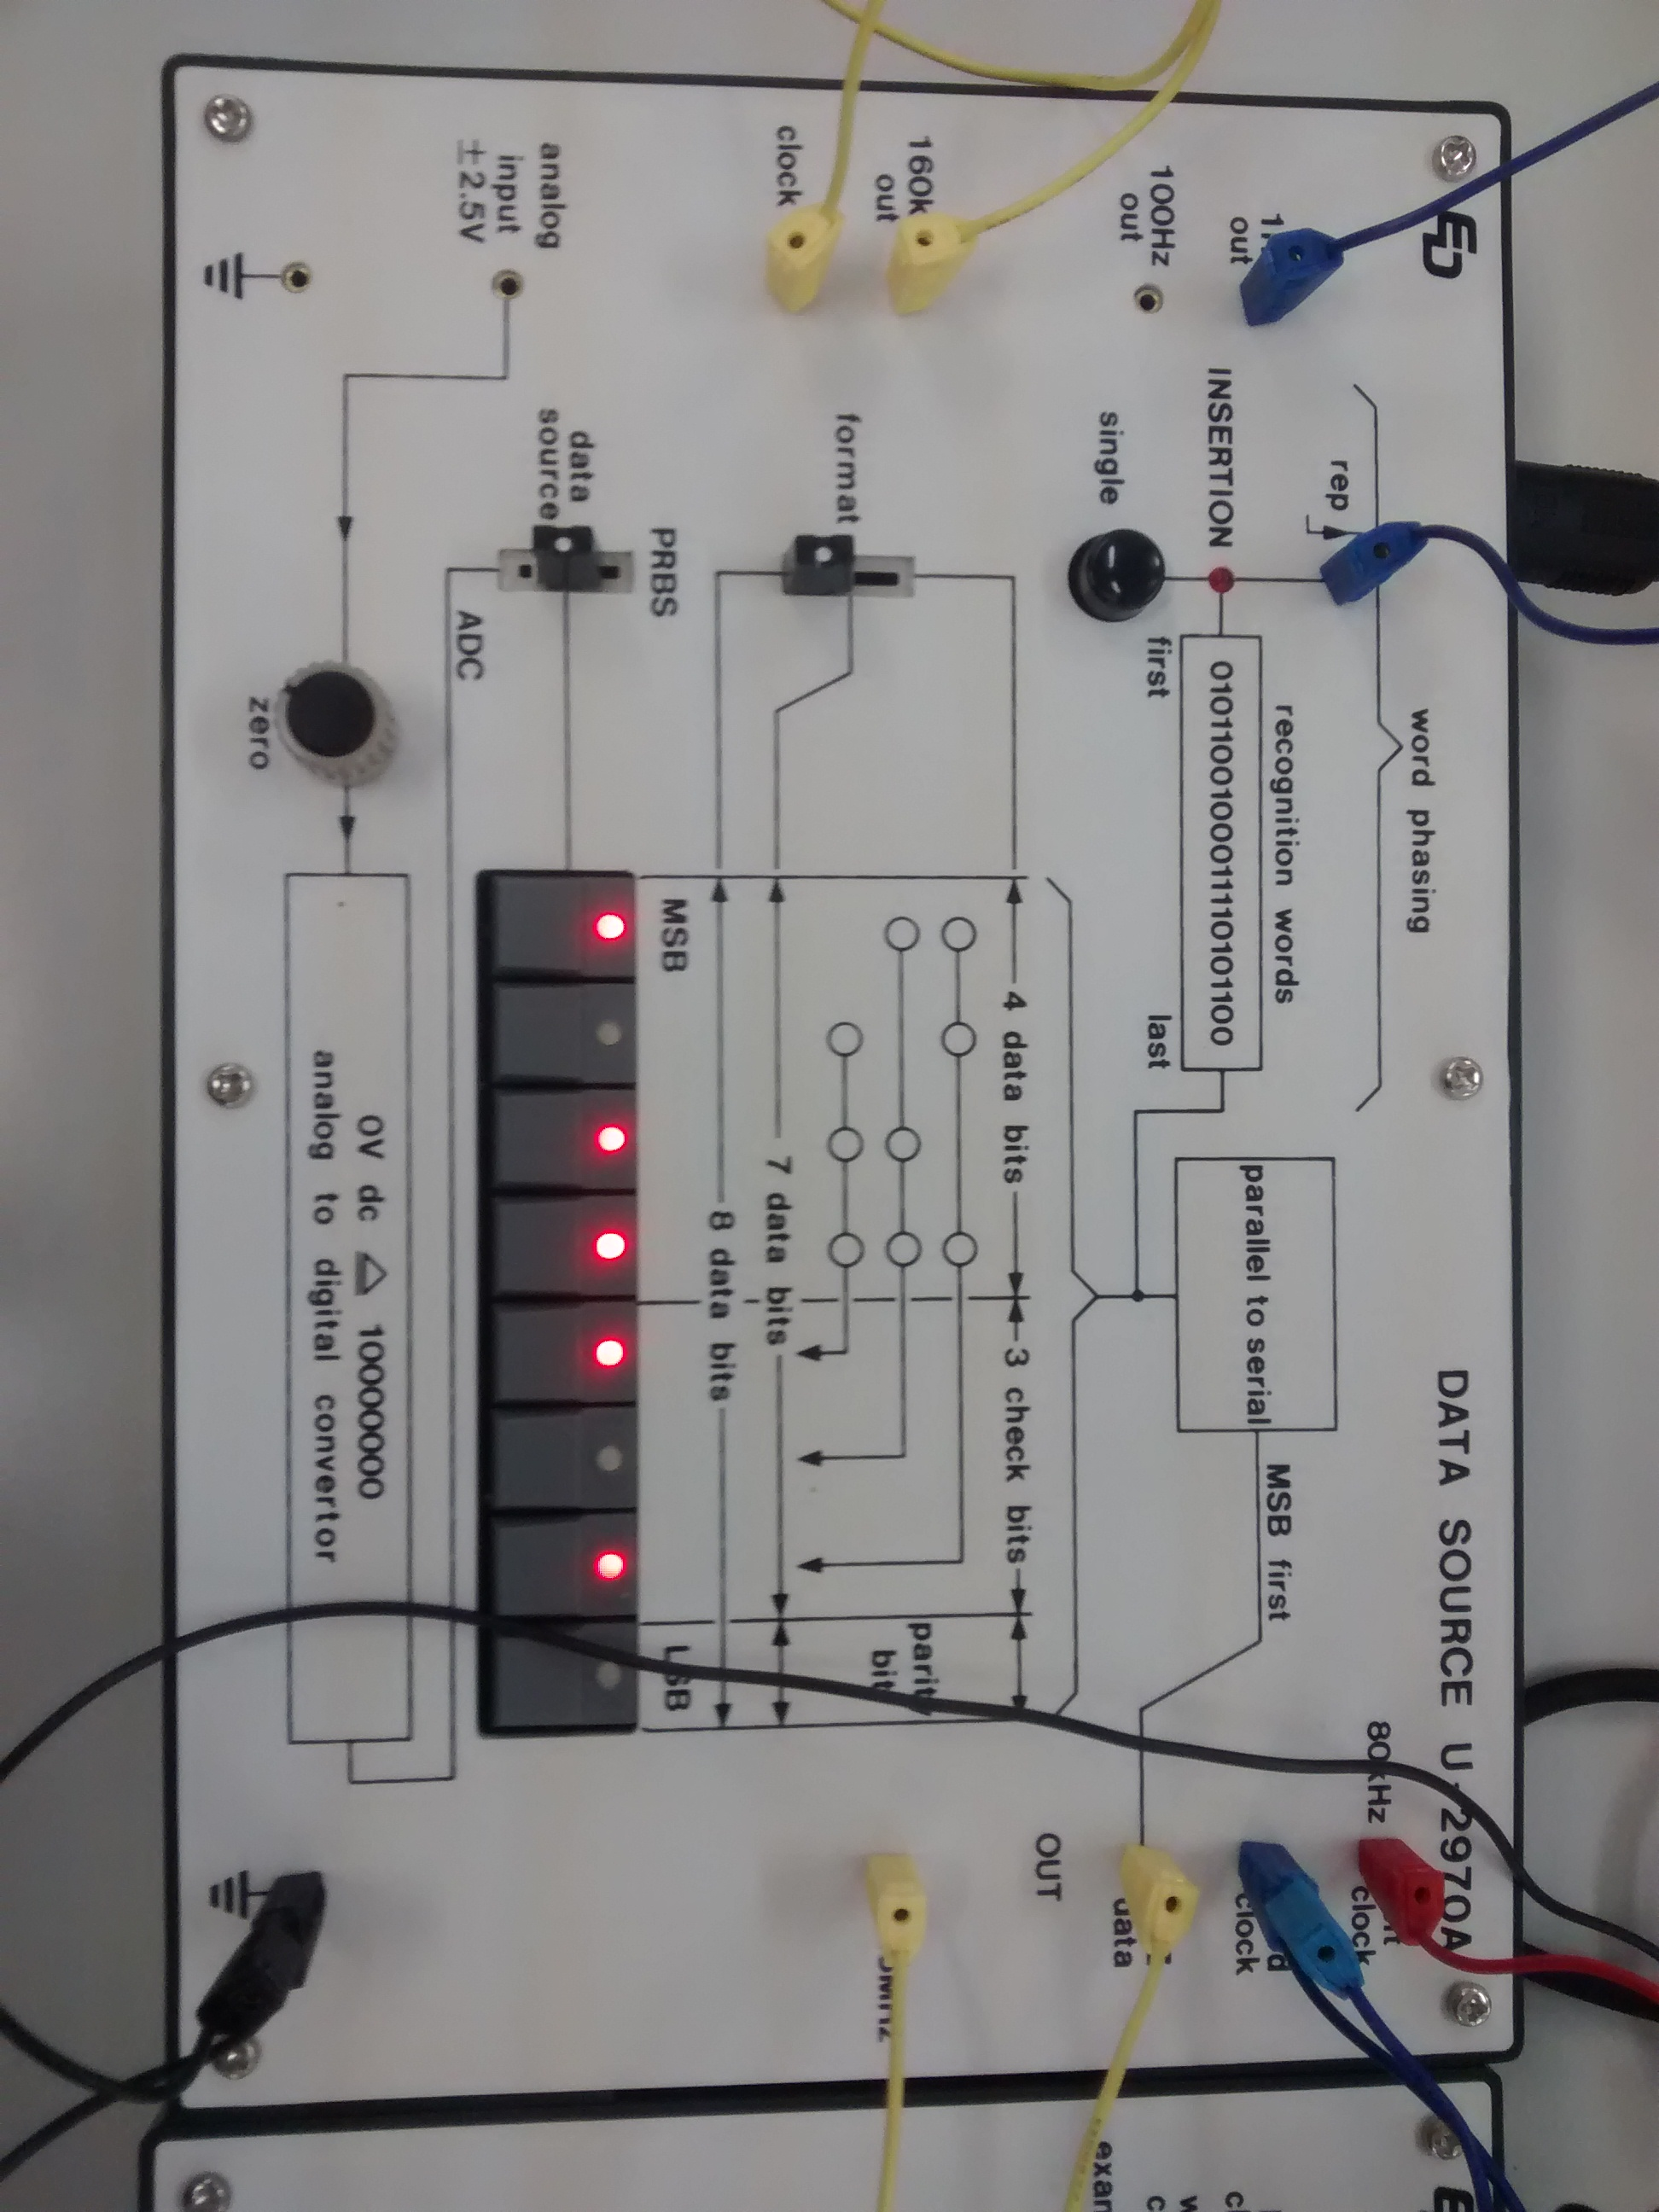
\includegraphics[scale=0.8]{montagem1}
  
  \small Fonte: Autoria própria.
  \label{fig:montagem1}
\end{figure}

Em seguida foram examinas as formas de onda para o sinal \emph{A} e \emph{B}, onde foi constatado que a onda \emph{A} possui os bits ímpares e a onda \emph{B} possui os bits pares, conforme mostram as figuras \ref{fig:osc1} e \ref{fig:osc2}, respectivamente.

\begin{figure}[H]
  \centering
  \caption{Forma de onda \emph{A}.}
  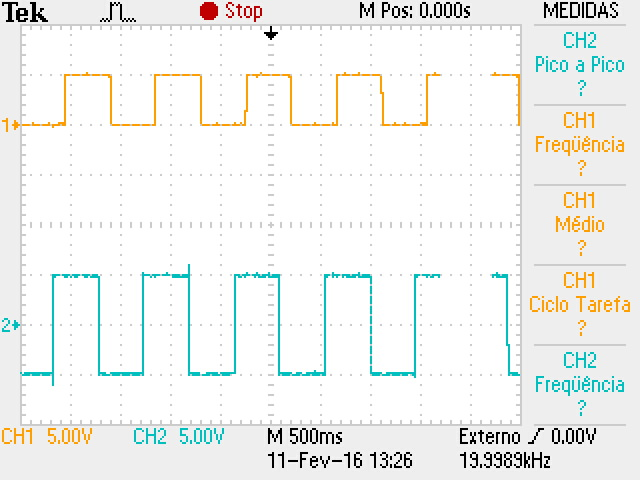
\includegraphics[scale=0.8]{osc1}
  
  \small Fonte: Autoria própria.
  \label{fig:osc1}
\end{figure}

\begin{figure}[H]
  \centering
  \caption{Forma de onda \emph{B}.}
  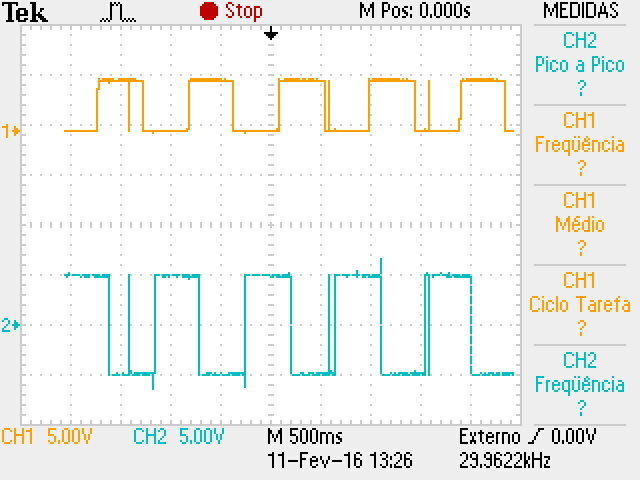
\includegraphics[scale=0.8]{osc2}
  
  \small Fonte: Autoria própria.
  \label{fig:osc2}
\end{figure}

Foi então investigada as formas de onda nos integradores \emph{A} e \emph{B}, conforme mostram as figuras \ref{fig:osc3} e \ref{fig:osc4}, respectivamente.

\begin{figure}[H]
  \centering
  \caption{Forma de onda do integrador \emph{A}.}
  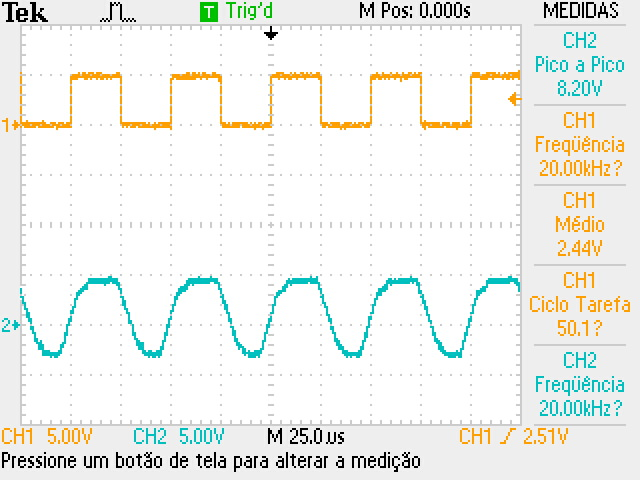
\includegraphics[scale=0.8]{osc4}
  
  \small Fonte: Autoria própria.
  \label{fig:osc3}
\end{figure}

\begin{figure}[H]
  \centering
  \caption{Forma de onda do integrador \emph{B}.}
  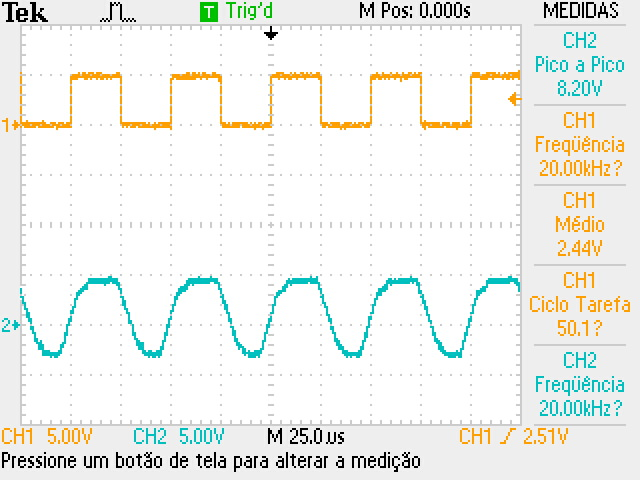
\includegraphics[scale=0.8]{osc4}
  
  \small Fonte: Autoria própria.
  \label{fig:osc4}
\end{figure}

Observou-se que a palavra é deslocada quando interrompemos o bit de clock. Também notou-se que a lampada A pisca para sinalizar o reconhecimento do deslocamento de palavra.

A montagem final é mostrada na figura \ref{fig:montagem2}.

\begin{figure}[H]
  \centering
  \caption{Montagem resultante para o primeiro experimento.}
  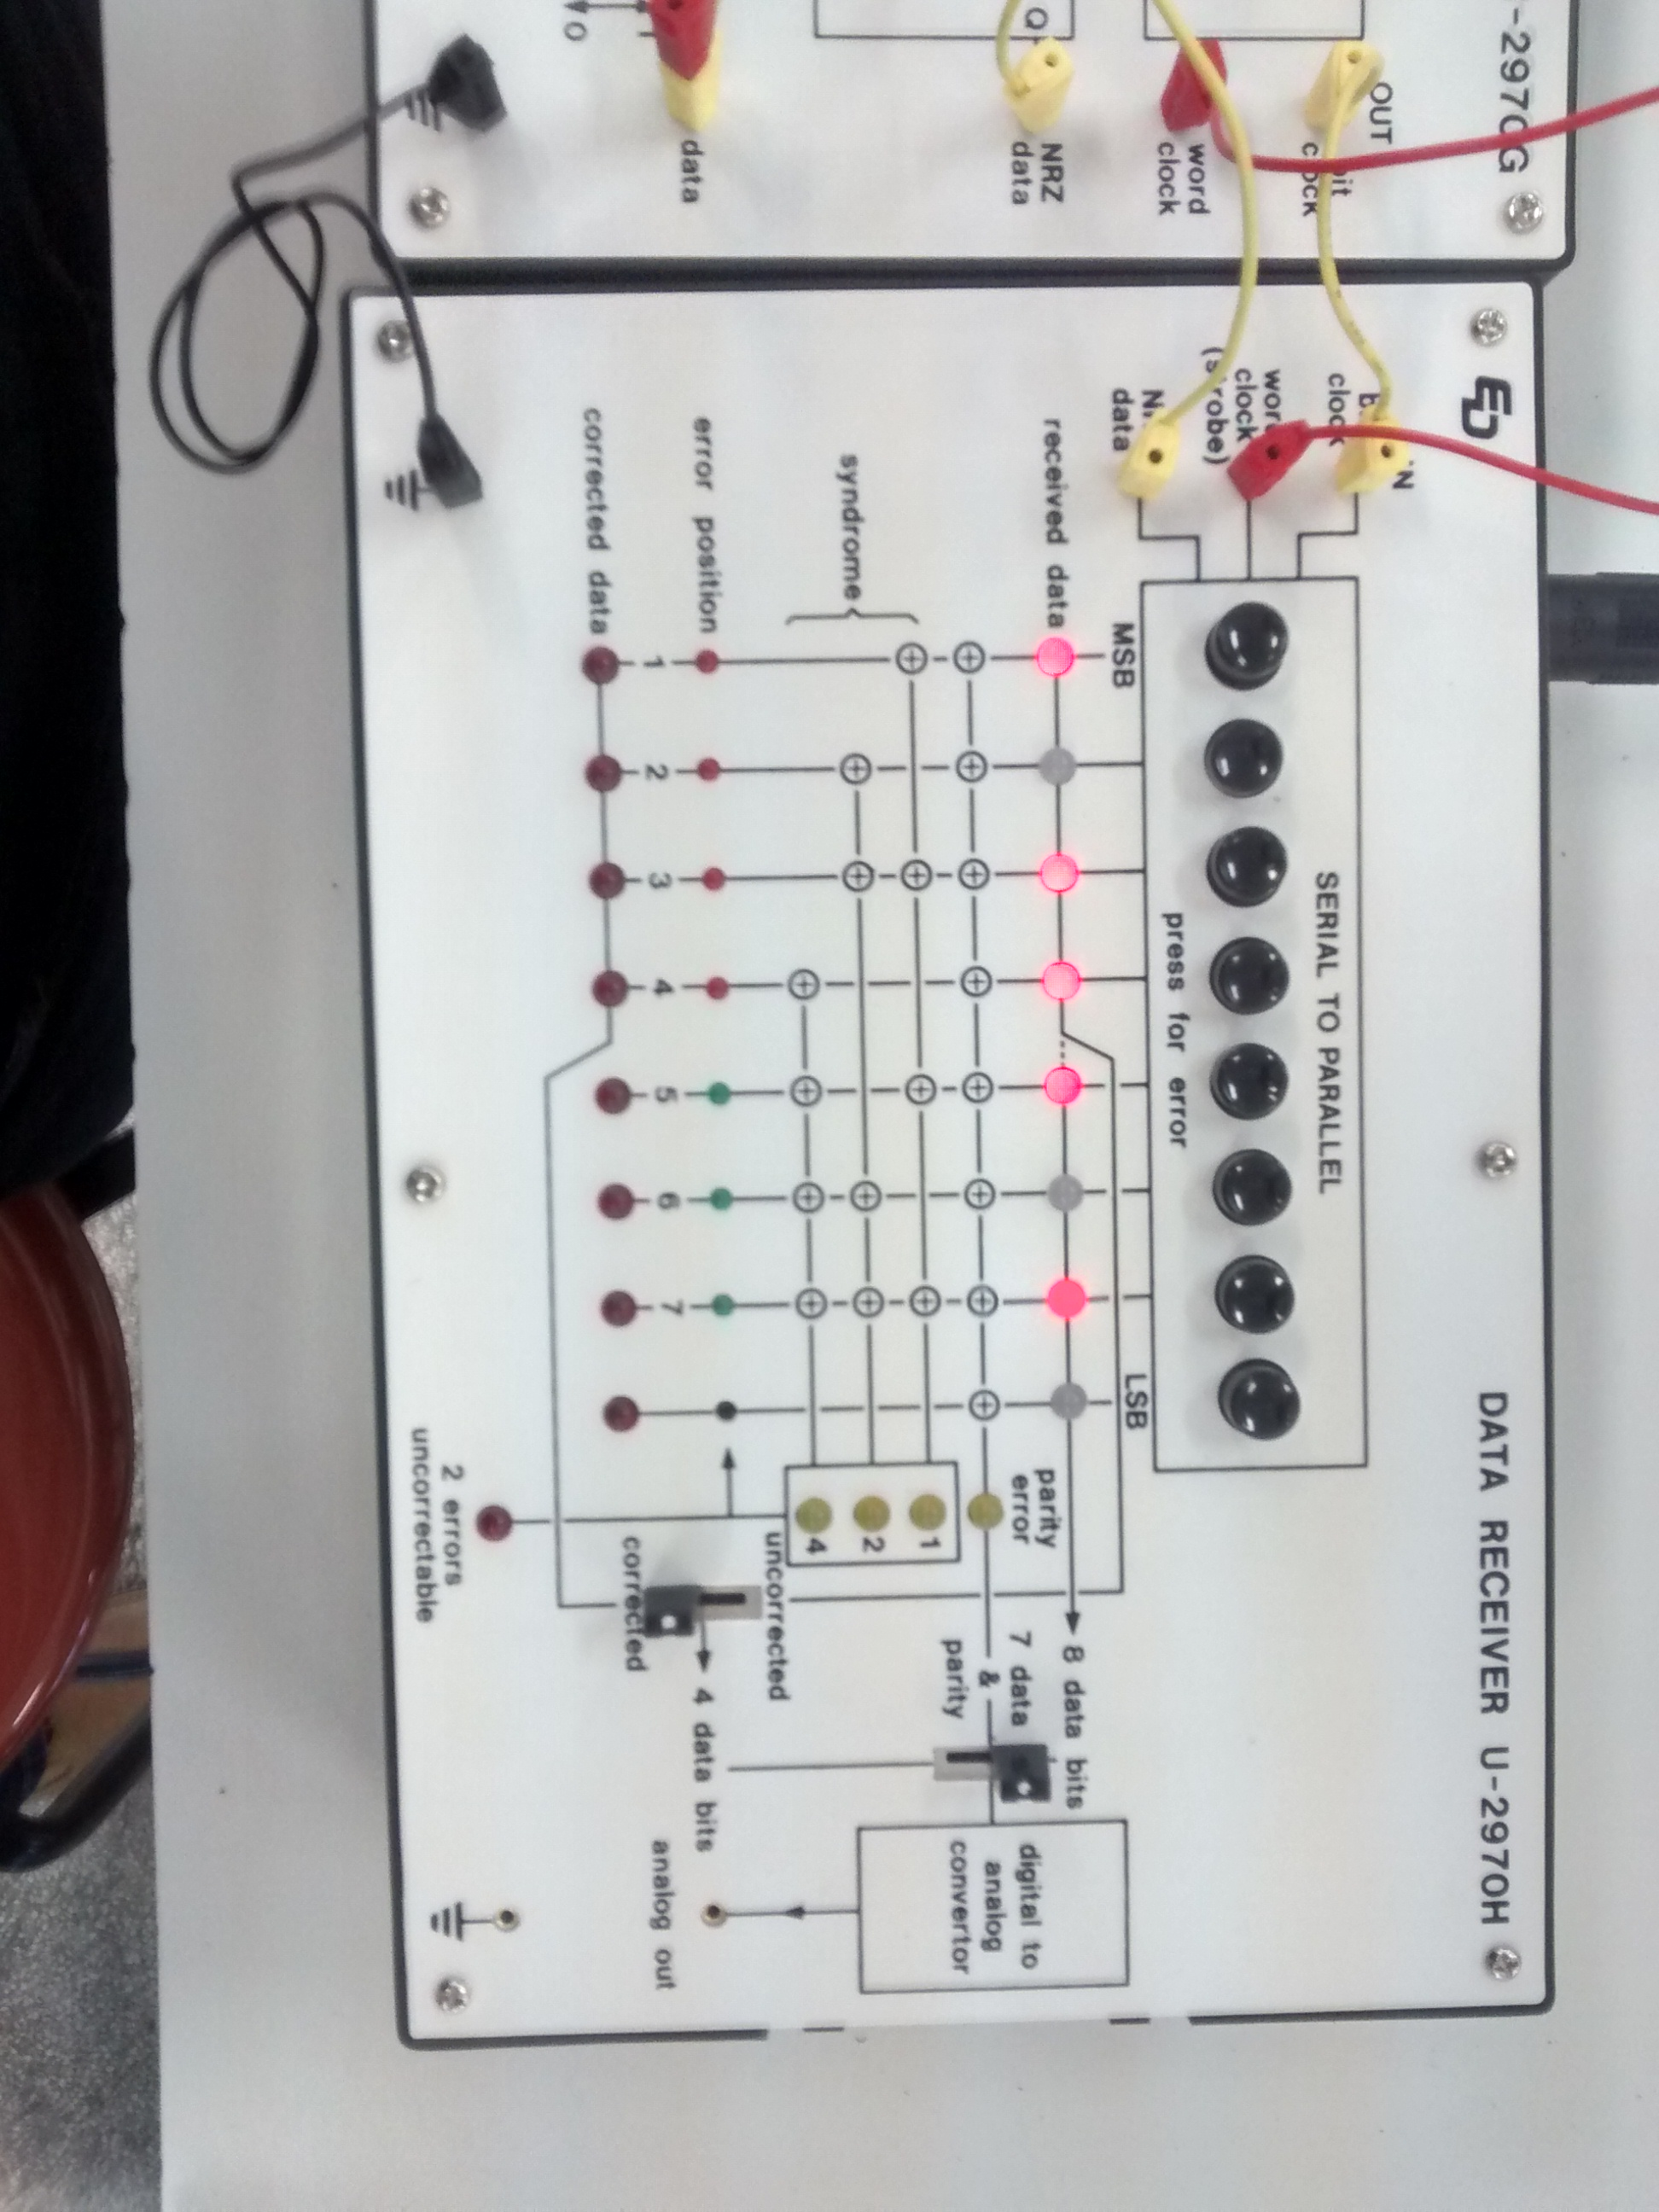
\includegraphics[scale=0.8]{montagem2}
  
  \small Fonte: Autoria própria.
  \label{fig:montagem2}
\end{figure}

\subsection{Método 2: Transmissão QSPK}

Para o método 2, primeiramente foi realizada a montagem, de acordo com a figura \ref{fig:montagem}-b, conforme mostra a figura \ref{fig:montagem3}.

\begin{figure}[H]
  \centering
  \caption{Montagem para o segundo experimento.}
  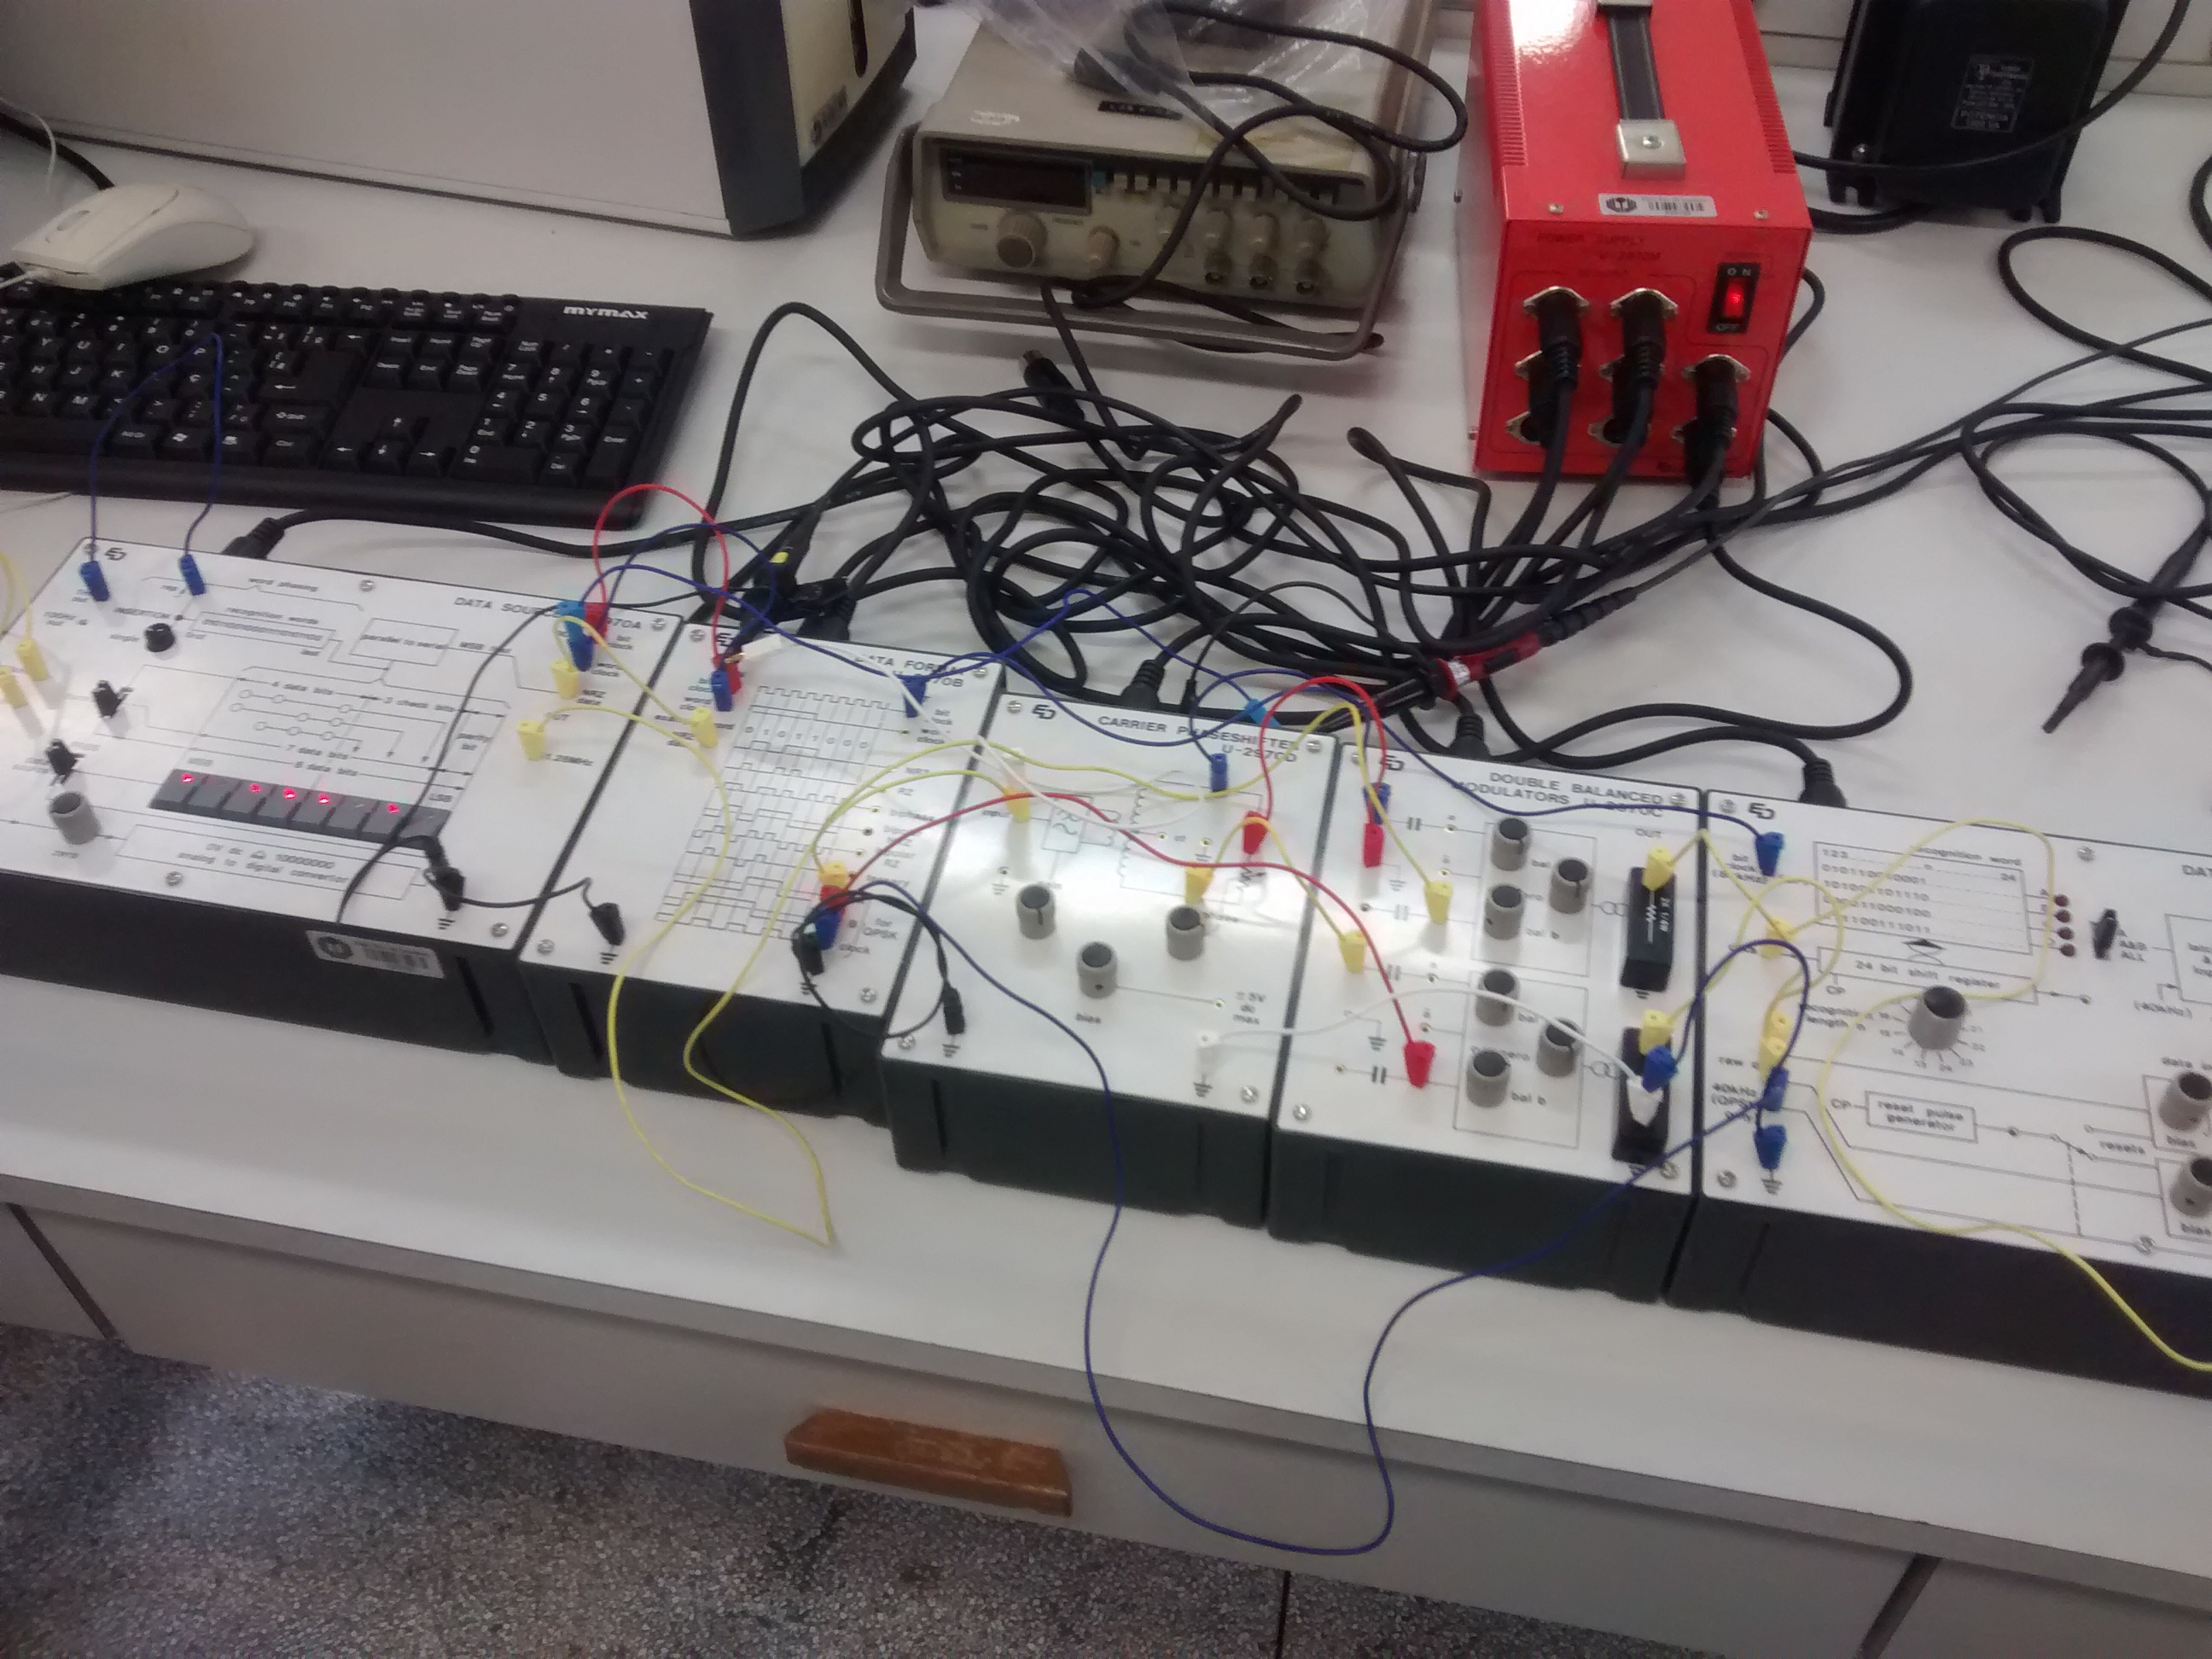
\includegraphics[scale=0.8]{montagem3}
  
  \small Fonte: Autoria própria.
  \label{fig:montagem3}
\end{figure}

Em seguida foi observado que os sinais estavam em quadratura, conforme mostra a figura \ref{fig:osc5}.

\begin{figure}[H]
  \centering
  \caption{Sinais em quadratura.}
  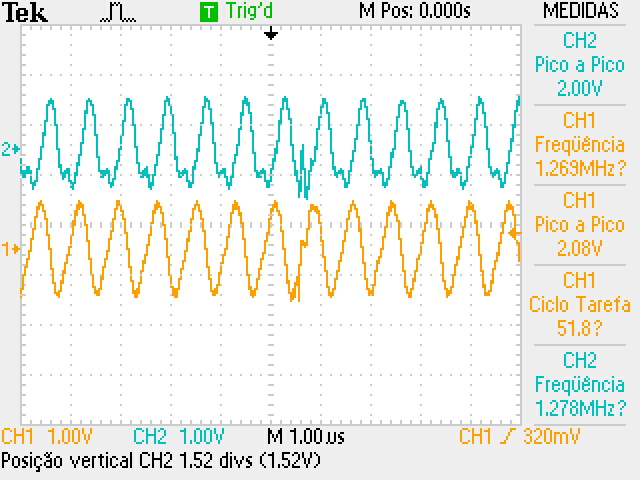
\includegraphics[scale=0.8]{osc5}
  
  \small Fonte: Autoria própria.
  \label{fig:osc5}
\end{figure}

Foram realizados os ajustes na montagem, como indicam os procedimentos 3 e 4. Observou-se que as duas senoides estavam em quadratura, como mostra a figura \ref{fig:osc6}.

\begin{figure}[H]
  \centering
  \caption{Senoides em quadratura.}
  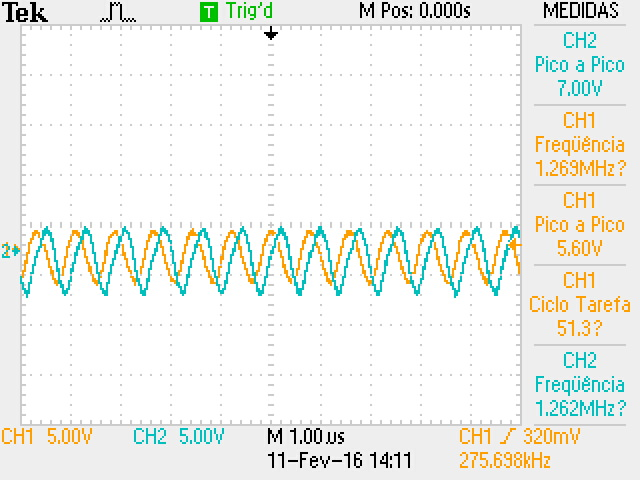
\includegraphics[scale=0.8]{osc6}
  
  \small Fonte: Autoria própria.
  \label{fig:osc6}
\end{figure}

Após as modificações dos itens 6 e 7, observou-se que a combinação impar muda o brilho do modulador superior e que a combinação par inverte a fase do modulador inferior.

Para visualizar a inversão de fase, os primeiros bits foram colocados em 00 (figura \ref{fig:osc7}) e em seguida em 11 (figura \ref{fig:osc8}). Fica evidente a inversão de fases.

\begin{figure}[H]
  \centering
  \caption{Bits 00000000.}
  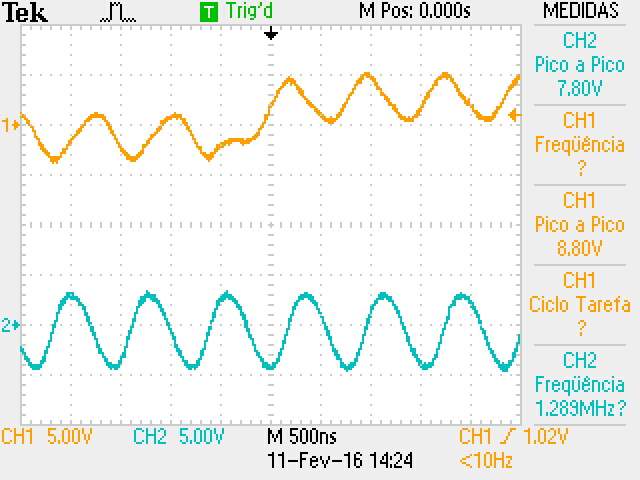
\includegraphics[scale=0.8]{osc7}
  
  \small Fonte: Autoria própria.
  \label{fig:osc7}
\end{figure}

\begin{figure}[H]
  \centering
  \caption{Bits 11000000.}
  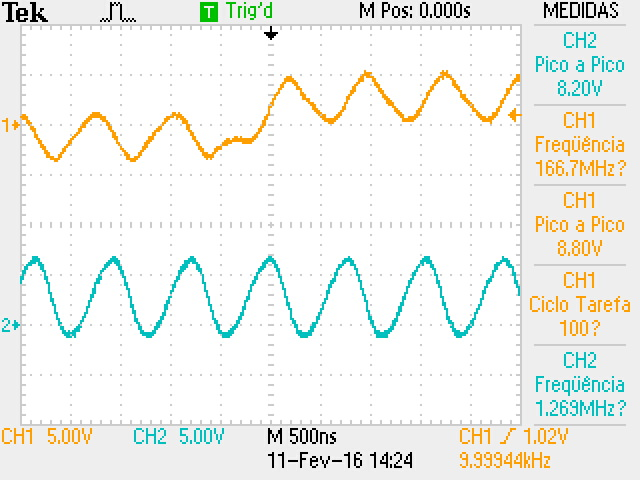
\includegraphics[scale=0.8]{osc8}
  
  \small Fonte: Autoria própria.
  \label{fig:osc8}
\end{figure}

Após as mudanças necessárias (itens 8-11) foram observados os sinais em 4 configurações diferentes, mostrados nas figuras \ref{fig:osc9}, \ref{fig:osc10}, \ref{fig:osc11} e \ref{fig:osc12}.

\begin{figure}[H]
  \centering
  \caption{Bits 00000000.}
  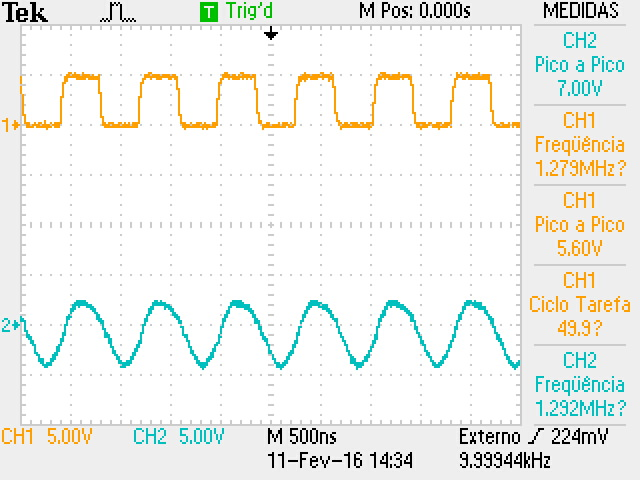
\includegraphics[scale=0.8]{osc9}
  
  \small Fonte: Autoria própria.
  \label{fig:osc9}
\end{figure}

\begin{figure}[H]
  \centering
  \caption{Bits 11111111.}
  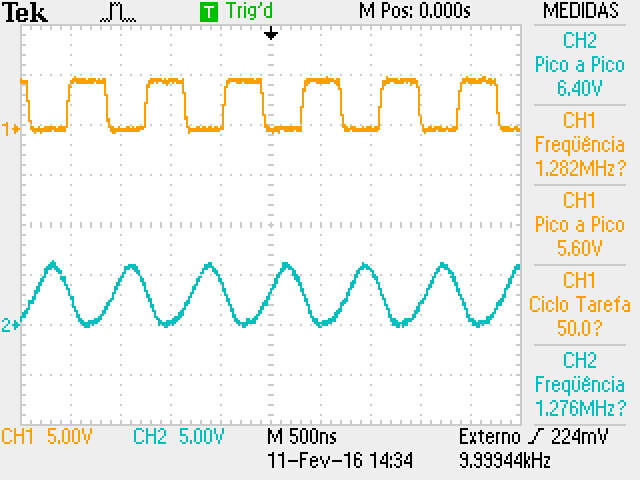
\includegraphics[scale=0.8]{osc10}
  
  \small Fonte: Autoria própria.
  \label{fig:osc10}
\end{figure}

\begin{figure}[H]
  \centering
  \caption{Bits 01010101.}
  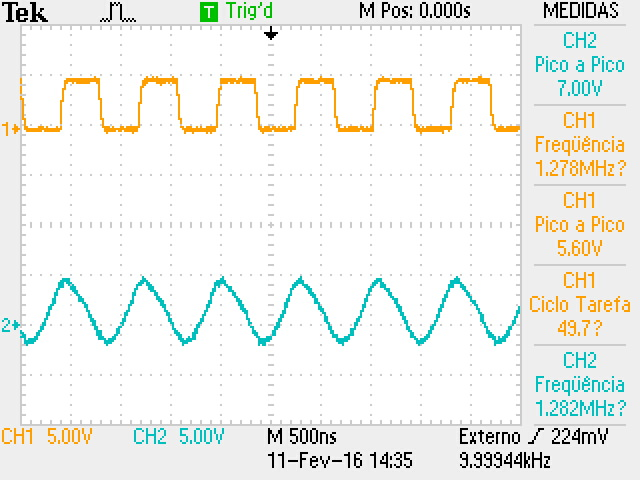
\includegraphics[scale=0.8]{osc11}
  
  \small Fonte: Autoria própria.
  \label{fig:osc11}
\end{figure}

\begin{figure}[H]
  \centering
  \caption{Bits 10101010.}
  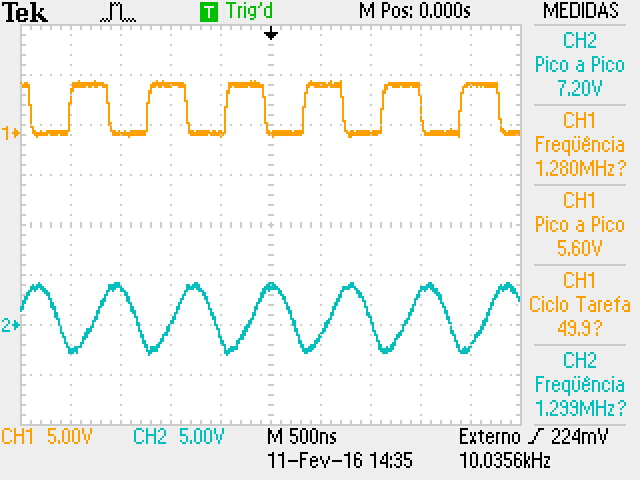
\includegraphics[scale=0.8]{osc12}
  
  \small Fonte: Autoria própria.
  \label{fig:osc12}
\end{figure}

Foi possível ver a forma de onda de saída que passando ciclicamente através de todas as suas quatro fases possíveis.

A figura \ref{fig:montagem4} mostra como ficou a montagem final.

\begin{figure}[H]
  \centering
  \caption{Montagem resultante para o segundo experimento.}
  \includegraphics[scale=0.8]{montagem4}
  
  \small Fonte: Autoria própria.
  \label{fig:montagem4}
\end{figure}

Por ultimo, a tabela \ref{tab:fases} mostra a relação entre o parte bits de dados e a fase das ondas, relativa a referência do canal 1 do osciloscópio.

\begin{table}[H]
  \centering
  \caption{Relação entre par de bits e fase.}
  \label{tab:fases}
  \begin{tabular}{cc}
    \toprule
    Bits & Fase [°] \\
    \midrule
    00 & 45 \\
    01 & 135 \\
    10 & 315 \\
    11 & 225 \\
    \bottomrule
  \end{tabular}
  
  \small Fonte: Autoria própria.
\end{table}
